\begin{frame}
	\frametitle{Atmosphäre - Luftmassen}

	\begin{figure}
		\centering
		\begin{tikzpicture}
			\node (image1) {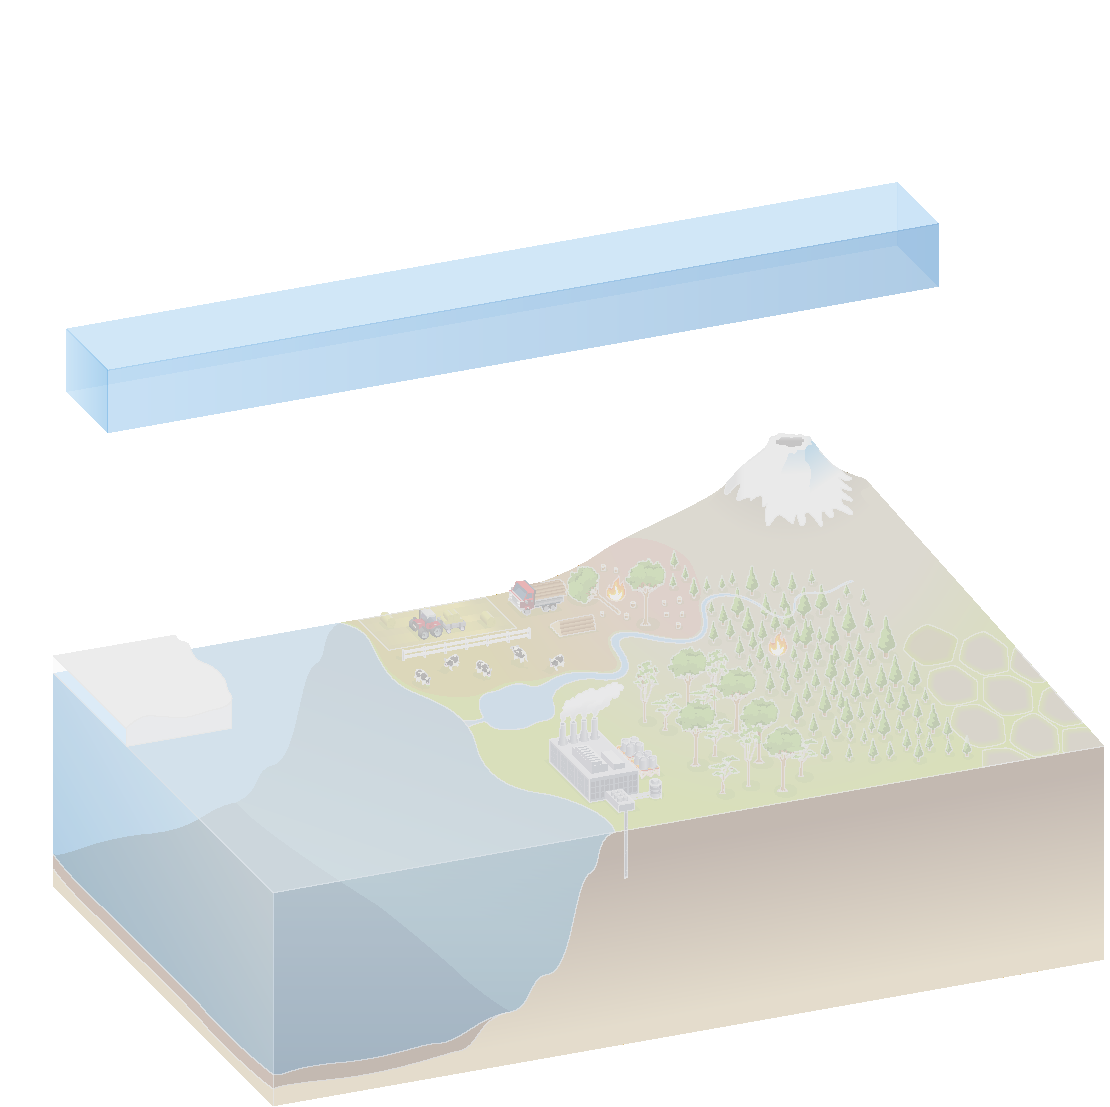
\includegraphics[trim={1cm 0cm 0cm 3cm}, clip, width=0.55\linewidth]{%
        	bilder/climate_components/global_climate_components_atmosphere.pdf}};
			\onslide<2|handout:0>\node (image2) at (image1.east) [xshift=-0.9cm]{%
					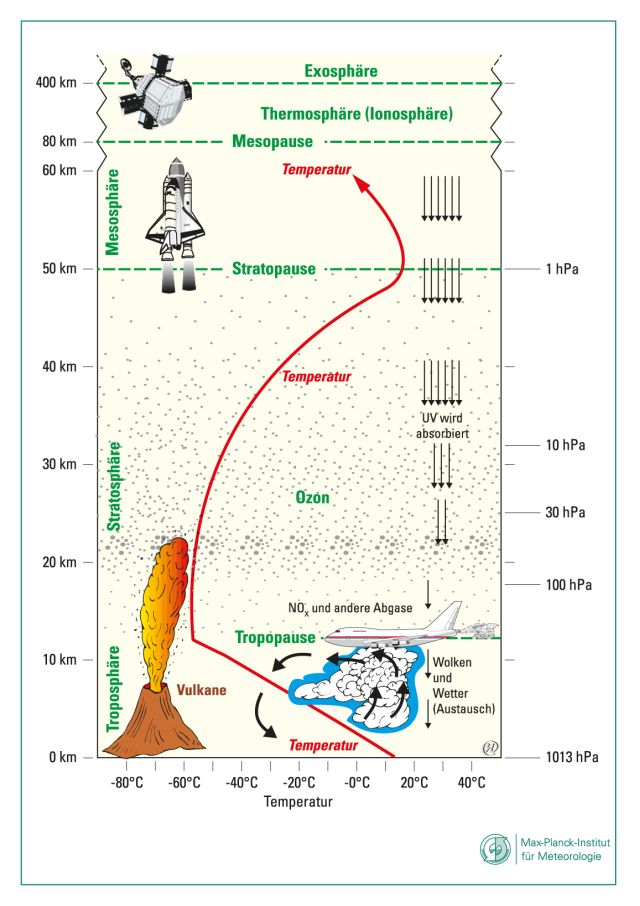
\includegraphics[width=0.35\linewidth] der Atmosphärenmasse, enthält fast allen Wasserdampf
			    \item[] Hier finden alle wetterrelevanten Phänomene statt
			  \end{itemize}
			  \item Stratosphäre, \SIrange{12}{50}{km}, \SIrange{-60}{0}{\celsius}, Ozon sorgt für Temperaturanstieg durch UV-Absorption
			  \item Mesosphäre, \SIrange{50}{80}{km}, \SIrange{-100}{0}{\celsius}, Temperatur fällt
			  \item Thermosphäre, \SIrange{80}{400}{km}, extrem geringe Teilchendichte, daher Temperatur nicht bestimmbar, Weltraum
			  \item Exosphäre, \SIrange{400}{1000}{km}, quasi Vakuum
			\end{itemize}
			\item[] Passt sich am schnellsten an Änderungen an
			\item[] in der planetaren Grenzschicht (\SIrange{1}{2.5}{km}): Reibung wichtig $\rightarrow$ starke vertikale Unterschiede in diesem Bereich der Atmosphäre
		\end{itemize}
		}
\end{frame}
